\documentclass{standalone}
\usepackage{tikz}
\usetikzlibrary{patterns, positioning}
\usepackage[sfdefault]{ClearSans} %% option 'sfdefault' activates Clear Sans as the default text font
\usepackage[T1]{fontenc}

\begin{document}
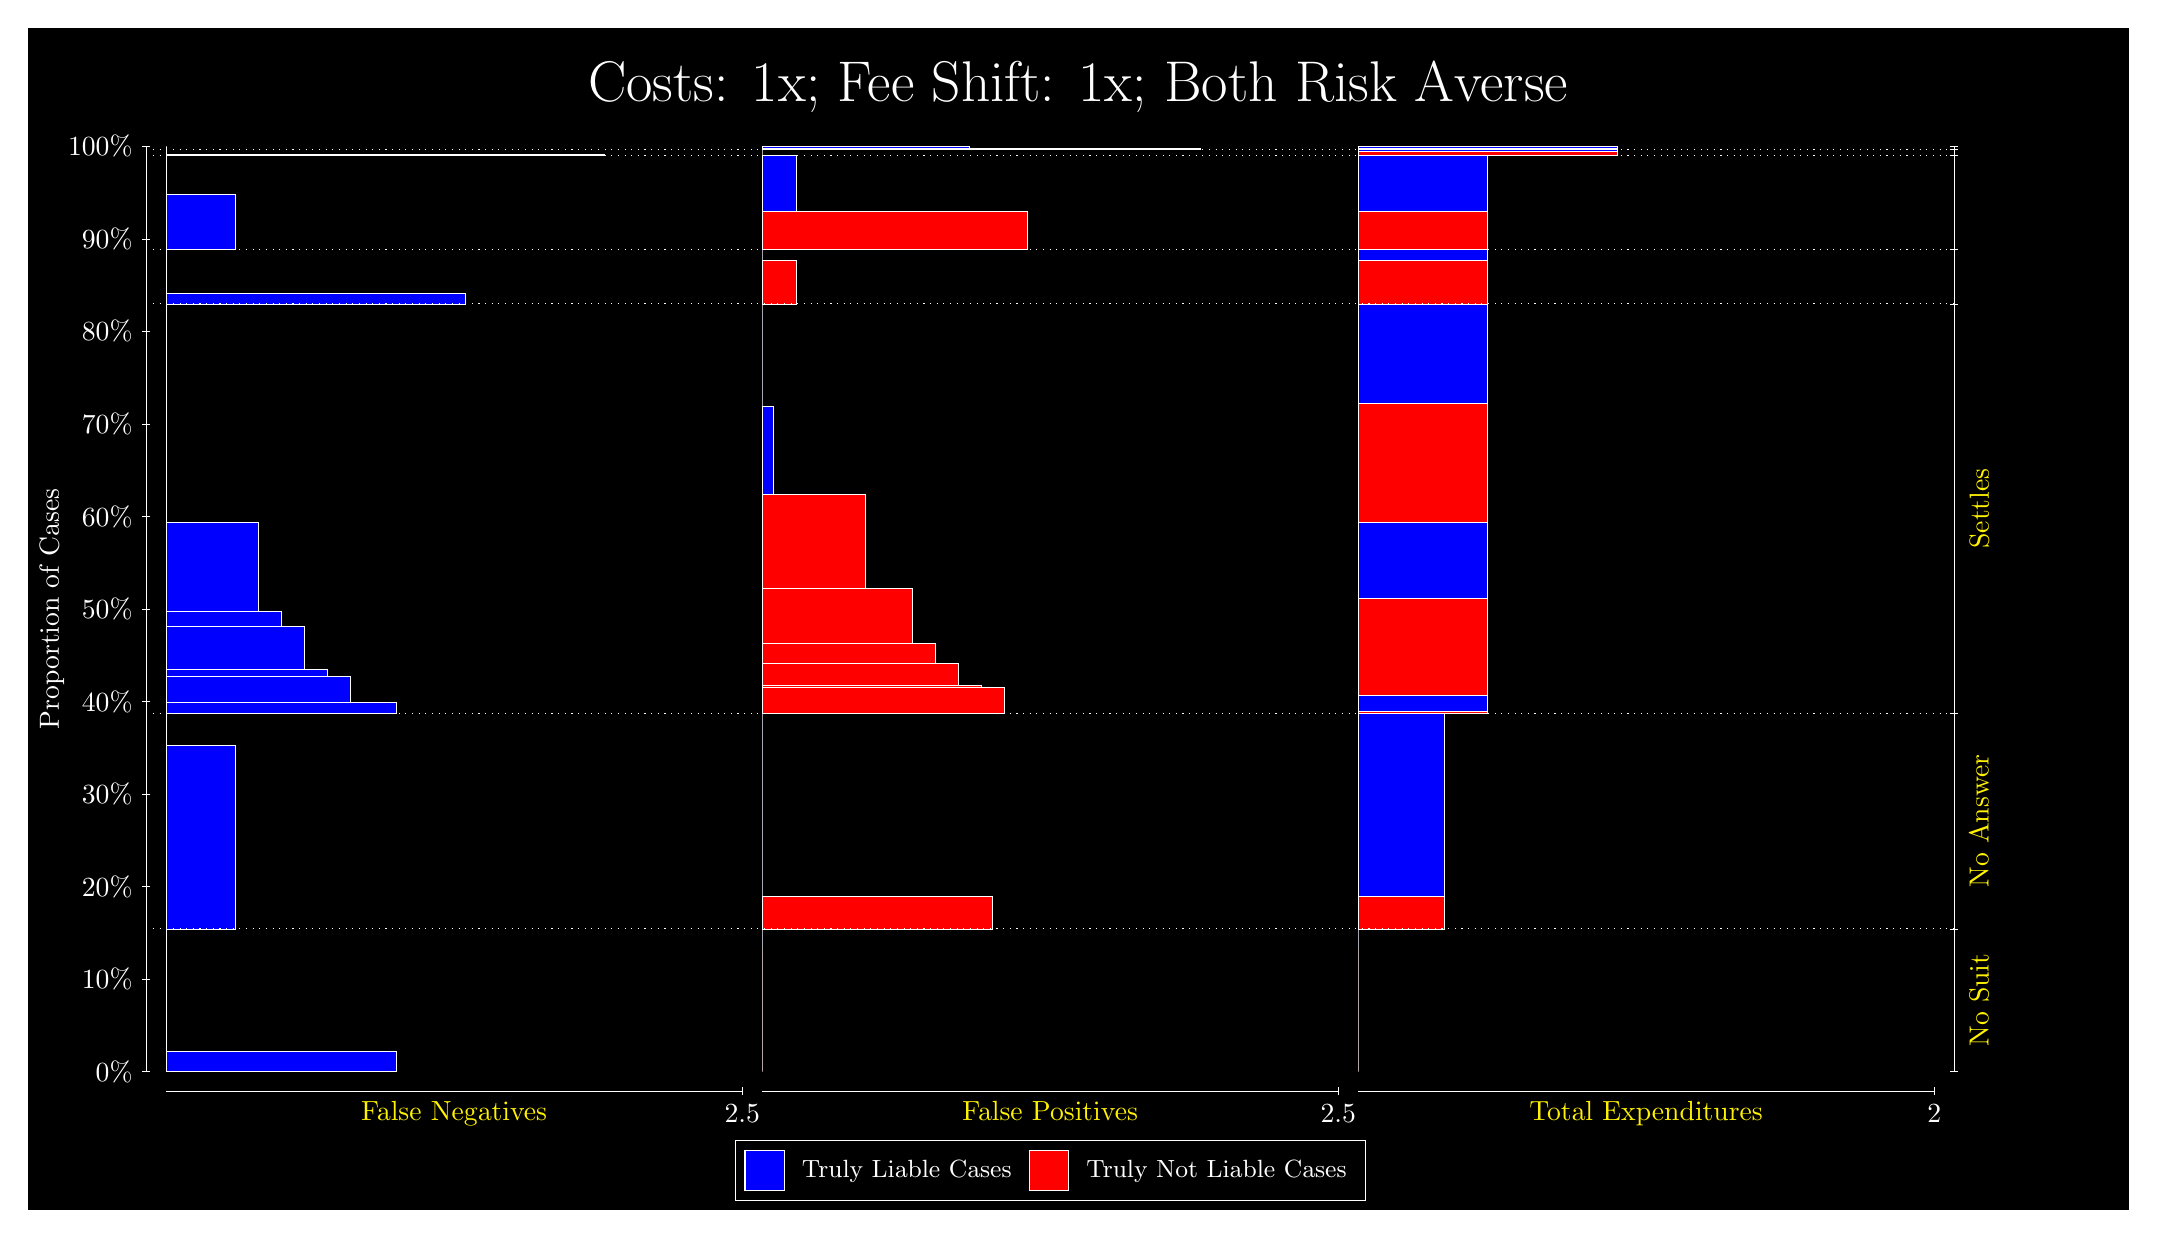
\begin{tikzpicture}
\draw[fill=black] (0,0) rectangle (26.667,15);
\draw[text=white] (0,13.5) rectangle (26.667,15) node[midway] {\huge Costs: 1x; Fee Shift: 1x; Both Risk Averse};
\draw[white, very thin] (1.5,1.75) -- (1.5,13.5);
\node[rotate=90, text=white, anchor=center] at (0.3, 7.625) {Proportion of Cases};
\draw[white, very thin] (1.45,1.75) -- (1.55,1.75);
\node[text=white, anchor=east] at (1.45, 1.75) {0\%};
\draw[white, very thin] (1.45,2.925) -- (1.55,2.925);
\node[text=white, anchor=east] at (1.45, 2.925) {10\%};
\draw[white, very thin] (1.45,4.1) -- (1.55,4.1);
\node[text=white, anchor=east] at (1.45, 4.1) {20\%};
\draw[white, very thin] (1.45,5.275) -- (1.55,5.275);
\node[text=white, anchor=east] at (1.45, 5.275) {30\%};
\draw[white, very thin] (1.45,6.45) -- (1.55,6.45);
\node[text=white, anchor=east] at (1.45, 6.45) {40\%};
\draw[white, very thin] (1.45,7.625) -- (1.55,7.625);
\node[text=white, anchor=east] at (1.45, 7.625) {50\%};
\draw[white, very thin] (1.45,8.8) -- (1.55,8.8);
\node[text=white, anchor=east] at (1.45, 8.8) {60\%};
\draw[white, very thin] (1.45,9.975) -- (1.55,9.975);
\node[text=white, anchor=east] at (1.45, 9.975) {70\%};
\draw[white, very thin] (1.45,11.15) -- (1.55,11.15);
\node[text=white, anchor=east] at (1.45, 11.15) {80\%};
\draw[white, very thin] (1.45,12.325) -- (1.55,12.325);
\node[text=white, anchor=east] at (1.45, 12.325) {90\%};
\draw[white, very thin] (1.45,13.5) -- (1.55,13.5);
\node[text=white, anchor=east] at (1.45, 13.5) {100\%};

\draw[white, very thin] (24.457,1.75) -- (24.457,13.5);
\draw[white, very thin] (24.407,1.75) -- (24.507,1.75);
\node[anchor=west] at (24.407, 1.75) {};
\draw[white, very thin] (24.407,3.5609) -- (24.507,3.5609);
\node[anchor=west] at (24.407, 3.5609) {};
\draw[white, very thin] (24.407,6.3018) -- (24.507,6.3018);
\node[anchor=west] at (24.407, 6.3018) {};
\draw[white, very thin] (24.407,11.5) -- (24.507,11.5);
\node[anchor=west] at (24.407, 11.5) {};
\draw[white, very thin] (24.407,12.188) -- (24.507,12.188);
\node[anchor=west] at (24.407, 12.188) {};
\draw[white, very thin] (24.407,13.38) -- (24.507,13.38);
\node[anchor=west] at (24.407, 13.38) {};
\draw[white, very thin] (24.407,13.461) -- (24.507,13.461);
\node[anchor=west] at (24.407, 13.461) {};
\draw[white, very thin] (24.407,13.5) -- (24.507,13.5);
\node[anchor=west] at (24.407, 13.5) {};

\draw[white, very thin, fill=blue] (1.75,1.75) rectangle (4.6775,2.0032);
\draw[white, very thin, fill=red] (1.75,2.0032) rectangle (1.75,3.5609);
\draw[white, very thin, fill=blue] (1.75,3.5609) rectangle (2.6283,5.8906);
\draw[white, very thin, fill=red] (1.75,5.8906) rectangle (1.75,6.3018);
\draw[white, very thin, fill=blue] (1.75,6.3018) rectangle (4.6775,6.4427);
\draw[white, very thin, fill=blue] (1.75,6.4427) rectangle (4.092,6.7635);
\draw[white, very thin, fill=blue] (1.75,6.7635) rectangle (3.7993,6.8526);
\draw[white, very thin, fill=blue] (1.75,6.8526) rectangle (3.5065,7.4041);
\draw[white, very thin, fill=blue] (1.75,7.4041) rectangle (3.2138,7.5998);
\draw[white, very thin, fill=blue] (1.75,7.5998) rectangle (2.921,8.7265);
\draw[white, very thin, fill=red] (1.75,8.7265) rectangle (1.75,11.5);
\draw[white, very thin, fill=blue] (1.75,11.5) rectangle (5.5558,11.629);
\draw[white, very thin, fill=red] (1.75,11.629) rectangle (1.75,12.188);
\draw[white, very thin, fill=blue] (1.75,12.188) rectangle (2.6283,12.886);
\draw[white, very thin, fill=red] (1.75,12.886) rectangle (1.75,13.38);
\draw[white, very thin, fill=blue] (1.75,13.38) rectangle (7.3123,13.397);
\draw[white, very thin, fill=red] (1.75,13.397) rectangle (1.75,13.461);
\draw[white, very thin, fill=red] (1.75,13.461) rectangle (1.75,13.478);
\draw[white, very thin, fill=blue] (1.75,13.478) rectangle (1.75,13.5);
\draw[white, very thin, fill=red] (9.3189,1.75) rectangle (9.3189,3.3077);
\draw[white, very thin, fill=blue] (9.3189,3.3077) rectangle (9.3189,3.5609);
\draw[white, very thin, fill=red] (9.3189,3.5609) rectangle (12.246,3.9721);
\draw[white, very thin, fill=blue] (9.3189,3.9721) rectangle (9.3189,6.3018);
\draw[white, very thin, fill=red] (9.3189,6.3018) rectangle (12.393,6.6243);
\draw[white, very thin, fill=red] (9.3189,6.6243) rectangle (12.1,6.651);
\draw[white, very thin, fill=red] (9.3189,6.651) rectangle (11.807,6.93);
\draw[white, very thin, fill=red] (9.3189,6.93) rectangle (11.515,7.1851);
\draw[white, very thin, fill=red] (9.3189,7.1851) rectangle (11.222,7.8867);
\draw[white, very thin, fill=red] (9.3189,7.8867) rectangle (10.636,9.0751);
\draw[white, very thin, fill=blue] (9.3189,9.0751) rectangle (9.4652,10.202);
\draw[white, very thin, fill=blue] (9.3189,10.202) rectangle (9.3189,11.5);
\draw[white, very thin, fill=red] (9.3189,11.5) rectangle (9.758,12.058);
\draw[white, very thin, fill=blue] (9.3189,12.058) rectangle (9.3189,12.188);
\draw[white, very thin, fill=red] (9.3189,12.188) rectangle (12.686,12.681);
\draw[white, very thin, fill=blue] (9.3189,12.681) rectangle (9.758,13.38);
\draw[white, very thin, fill=red] (9.3189,13.38) rectangle (9.3189,13.443);
\draw[white, very thin, fill=blue] (9.3189,13.443) rectangle (9.3189,13.461);
\draw[white, very thin, fill=red] (9.3189,13.461) rectangle (14.881,13.478);
\draw[white, very thin, fill=blue] (9.3189,13.478) rectangle (11.954,13.5);
\draw[white, very thin, fill=red] (16.888,1.75) rectangle (16.888,3.3077);
\draw[white, very thin, fill=blue] (16.888,3.3077) rectangle (16.888,3.5609);
\draw[white, very thin, fill=red] (16.888,3.5609) rectangle (17.986,3.9721);
\draw[white, very thin, fill=blue] (16.888,3.9721) rectangle (17.986,6.3018);
\draw[white, very thin, fill=red] (16.888,6.3018) rectangle (18.534,6.3285);
\draw[white, very thin, fill=blue] (16.888,6.3285) rectangle (18.534,6.5242);
\draw[white, very thin, fill=red] (16.888,6.5242) rectangle (18.534,7.7599);
\draw[white, very thin, fill=blue] (16.888,7.7599) rectangle (18.534,8.7212);
\draw[white, very thin, fill=red] (16.888,8.7212) rectangle (18.534,10.232);
\draw[white, very thin, fill=blue] (16.888,10.232) rectangle (18.534,11.5);
\draw[white, very thin, fill=red] (16.888,11.5) rectangle (18.534,12.058);
\draw[white, very thin, fill=blue] (16.888,12.058) rectangle (18.534,12.188);
\draw[white, very thin, fill=red] (16.888,12.188) rectangle (18.534,12.681);
\draw[white, very thin, fill=blue] (16.888,12.681) rectangle (18.534,13.38);
\draw[white, very thin, fill=red] (16.888,13.38) rectangle (20.181,13.443);
\draw[white, very thin, fill=blue] (16.888,13.443) rectangle (20.181,13.461);
\draw[white, very thin, fill=red] (16.888,13.461) rectangle (20.181,13.478);
\draw[white, very thin, fill=blue] (16.888,13.478) rectangle (20.181,13.5);
\draw[white, dotted] (1.5,3.5609) -- (24.457,3.5609);
\draw[white, dotted] (1.5,6.3018) -- (24.457,6.3018);
\draw[white, dotted] (1.5,11.5) -- (24.457,11.5);
\draw[white, dotted] (1.5,12.188) -- (24.457,12.188);
\draw[white, dotted] (1.5,13.38) -- (24.457,13.38);
\draw[white, dotted] (1.5,13.461) -- (24.457,13.461);
\draw[white, very thin] (1.75,1.5) -- (9.0689,1.5);
\node[text=yellow, anchor=north] at (5.4094, 1.5) {False Negatives};
\draw[white, very thin] (9.0689,1.45) -- (9.0689,1.55);
\node[text=white, anchor=north] at (9.0689, 1.45) {2.5};

\draw[white, very thin] (9.3189,1.5) -- (16.638,1.5);
\node[text=yellow, anchor=north] at (12.978, 1.5) {False Positives};
\draw[white, very thin] (16.638,1.45) -- (16.638,1.55);
\node[text=white, anchor=north] at (16.638, 1.45) {2.5};

\draw[white, very thin] (16.888,1.5) -- (24.207,1.5);
\node[text=yellow, anchor=north] at (20.547, 1.5) {Total Expenditures};
\draw[white, very thin] (24.207,1.45) -- (24.207,1.55);
\node[text=white, anchor=north] at (24.207, 1.45) {2};

\node[text=yellow, centered, rotate=90] at (24.777, 2.6555) {No Suit};
\node[text=yellow, centered, rotate=90] at (24.777, 4.9313) {No Answer};
\node[text=yellow, centered, rotate=90] at (24.777, 8.9008) {Settles};





\draw (12.978300999999998,1.5) node[draw=none] (baseCoordinate) {};
\begin{scope}[align=center]
        \matrix[scale=0.5, draw=white, below=0.5cm of baseCoordinate, nodes={draw}, column sep=0.1cm]{
            \node[rectangle, draw, minimum width=0.5cm, minimum height=0.5cm, fill=blue] {}; &
            \node[draw=none, font=\small, text=white] (B) {Truly Liable Cases}; &
            \node[rectangle, draw, minimum width=0.5cm, minimum height=0.5cm, fill=red] {}; &
            \node[draw=none, font=\small, text=white] (B) {Truly Not Liable Cases}; \\
            };
\end{scope}

\end{tikzpicture}
\end{document}